\chapter{लघुपथन और विद्युत सुरक्षा}\label{ch:g7:short-circuits-safety}

तुमने अब तक जो भी सुरक्षा-नियम सीखा है, उसका रास्ता उसी एक खलनायक तक
जाता है जिससे पिछले साल थोड़ी-सी मुलाक़ात हुई थी: \omterm{def:g7:short-circuits-safety:device}{लघुपथन}। यह अध्याय उसका
ठीक से अध्ययन करता है --- वह शुरू कैसे होता है, जलाता क्यों है, और एक
मामूली-सा क़ुरबान होने वाला तार उसे कैसे हरा देता है --- और घर की
फ़्यूज़-पेटी को रहस्यमय अलमारी से बदलकर ऐसा साथी बना देता है जिसे तुम
समझते हो।

\section{खलनायक का तरीक़ा}

\begin{proposition}[धारा को बिना मेहनत वाली सड़क पसंद है]\label{prop:g7:short-circuits-safety:effortless}
एक ही दो बिंदुओं को जोड़ती दो सड़कों में से चलती हुई धारा उसी पर भीड़
बना लेती है जो उसका कम विरोध करती है। उपकरण --- लैंप, \omterm{ex:g6:circuits-and-safety:motor}{मोटर}, \omterm{ex:g6:circuits-and-safety:motor}{बज़र} ---
काम करते हुए क़तार का विरोध करते हैं; और सादा मोटा तार लगभग विरोध करता
ही नहीं। क़तार को नंगे तार वाला बाईपास दे दो, और वह काम वाली सड़क
लगभग पूरी तरह छोड़कर उस बिना मेहनत वाली सड़क पर चली जाती है।
\end{proposition}

\begin{definition}[किसी उपकरण का लघुपथन]\label{def:g7:short-circuits-safety:device}
कोई उपकरण तब \emph{लघुपथित}\index{लघुपथन} होता है जब कोई \omterm{def:g4:conductors-insulators:conductor}{चालक} सड़क
उसके दोनों सिरों को सीधे जोड़ देती है और उसे छोड़ देती है। क़तार उपकरण
को त्याग देती है --- लघुपथित लैंप बुझ जाता है, \omterm{ex:g6:circuits-and-safety:motor}{मोटर} रुक जाती है ---
जबकि बाक़ी फंदा चलता रहता है, और अब क़तार का विरोध करने वाला एक
मज़दूर कम रह जाता है।
\end{definition}

\begin{definition}[बैटरी का लघुपथन]\label{def:g7:short-circuits-safety:battery}
सबसे भारी मामला: कोई \omterm{def:g4:conductors-insulators:conductor}{चालक} सड़क \emph{\omterm{def:g3:first-electric-circuit:battery}{बैटरी}} के दोनों सिरों को जोड़ दे
और उस पर कहीं कोई उपकरण न हो। तब क़तार का विरोध करने वाला कुछ बचता ही
नहीं, और वह भगदड़ बन जाती है --- यह बेतहाशा दौड़ तार को और ख़ुद \omterm{def:g3:first-electric-circuit:battery}{बैटरी}
को तपा देती है, सेल बरबाद कर देती है, \omterm{def:g4:conductors-insulators:insulator}{विद्युतरोधी} परत पिघला देती है,
और घर की बिजली में घरों को आग के हवाले कर देती है।
\end{definition}

\begin{method}[खलनायक का सुरक्षित प्रदर्शन]\label{met:g7:short-circuits-safety:demo}
एक \omterm{def:g3:first-electric-circuit:battery}{बैटरी} और \omterm{def:g4:series-circuits:series}{श्रेणी में} लगे दो बल्बों से (सुरक्षित: \omterm{def:g3:first-electric-circuit:battery}{बैटरी} का धक्का बहुत
हल्का है):
\begin{enumerate}
  \item दोनों \omterm{def:g3:first-electric-circuit:bulb}{बल्ब} जलाओ --- बराबर मंद, जैसा श्रेणी का नियम वादा करता
        है;
  \item अब एक सादा तार \omterm{def:g3:first-electric-circuit:bulb}{बल्ब} 2 के दोनों सिरों पर छुआकर उसे बाईपास कर
        दो;
  \item देखो: \omterm{def:g3:first-electric-circuit:bulb}{बल्ब} 2 उसी पल मर जाता है --- त्यागा हुआ --- जबकि \omterm{def:g3:first-electric-circuit:bulb}{बल्ब}
        1 और \emph{ज़्यादा चमकीला} हो जाता है: एक विरोधी के बाईपास
        होते ही पूरे फंदे की क़तार मज़बूत हो जाती है;
  \item तार हटा दो: क़तार फिर \omterm{def:g3:first-electric-circuit:bulb}{बल्ब} 2 में घुस जाती है, और बराबर मंदी
        लौट आती है।
\end{enumerate}
एक प्रयोग, तीन सबक़: बाईपास का नियम, त्यागा गया उपकरण, और मज़बूत हुई
दौड़।
\end{method}

\begin{omfigure}
\begin{tikzpicture}[scale=0.9]
  \draw (0,0) to[battery1, l=बैटरी] (0,2.8)
    to[short] (1.8,2.8)
    to[lamp, l=बल्ब 1: ज़्यादा चमकीला!] (4.4,2.8)
    to[lamp, l=बल्ब 2: अँधेरा] (7.0,2.8)
    to[short] (8.4,2.8)
    to[short] (8.4,0)
    to[short] (0,0);
  \draw[very thick, omThm] (4.7,2.8) to[bend left=48] (6.7,2.8);
  \node[above, font=\small, omThm] at (5.7,3.75)
    {बाईपास: क़तार बल्ब 2 को छोड़ देती है};
\end{tikzpicture}

{\small किसी उपकरण का \omterm{def:g7:short-circuits-safety:device}{लघुपथन}: \omterm{def:g3:first-electric-circuit:bulb}{बल्ब} 2 पर रखा नंगा तार उसकी पूरी क़तार
चुरा लेता है --- \omterm{def:g3:first-electric-circuit:bulb}{बल्ब} 2 मर जाता है, और \omterm{def:g3:first-electric-circuit:bulb}{बल्ब} 1, अब अकेला \omterm{def:g3:first-electric-circuit:battery}{बैटरी} के
सामने, ज़्यादा तेज़ जलता है।}
\end{omfigure}

\begin{example}[तार तपते क्यों हैं]\label{ex:g7:short-circuits-safety:heating}
चलती हुई धारा अपनी सड़क को हमेशा थोड़ा गरम करती है --- लैंप की दमक
वही गरमाहट है, जिसे जान-बूझकर काम पर लगाया गया है, और वह भी सफ़ेद-गरम
चलने के लिए बने तंतु में। भगदड़ में यही गरमाहट ख़तरा बन जाती है:
\omterm{def:g7:short-circuits-safety:device}{लघुपथन} की दौड़ ताँबे के तार को कुछ ही सेकंडों में उसकी प्लास्टिक परत के
\omterm{def:g4:changes-of-state:melting-point}{गलनांक} से भी ऊपर तपा सकती है। जेब भर का पूर्वाभास: तार से \omterm{def:g7:short-circuits-safety:device}{लघुपथित} की
गई \omterm{def:g3:first-electric-circuit:battery}{बैटरी} तुम्हारे हाथ में गरम हो जाती है --- और वही भौतिकी, घर की
बिजली के पैमाने पर, दीवारें झुलसा देती है। (दौड़ के साथ गरमाहट कैसे
बढ़ती है, यह दो साल बाद विद्युत शक्ति वाले अध्याय में ईमानदारी से मापा
जाता है।)
\end{example}

\begin{omfigure}
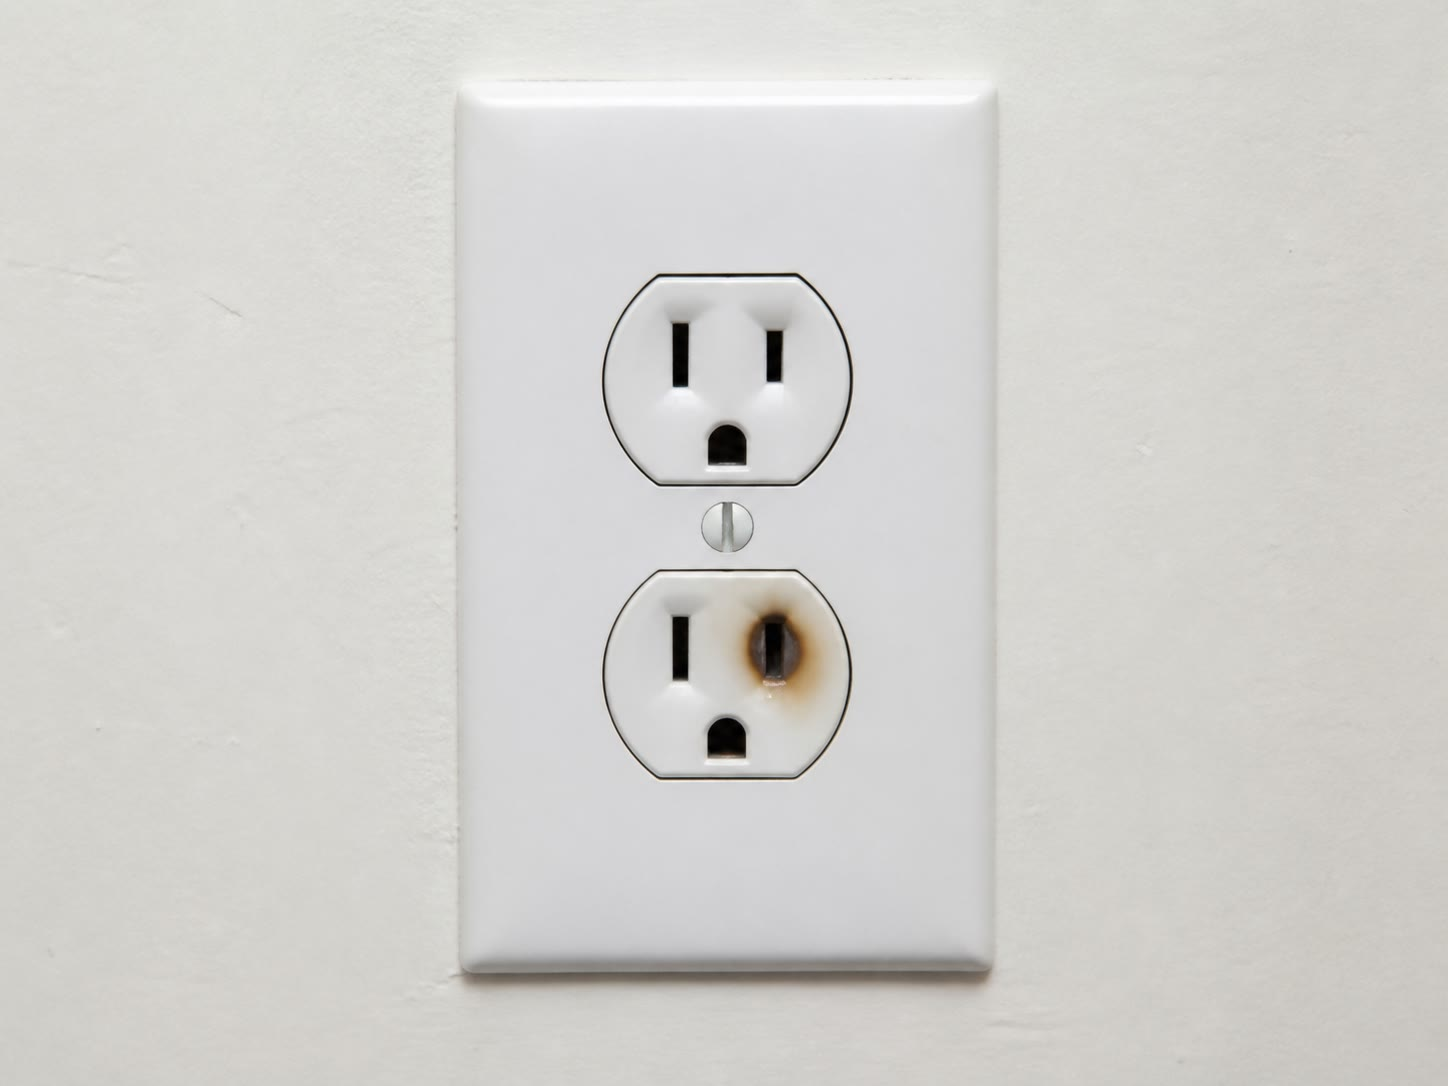
\includegraphics[width=0.45\linewidth]{images/book1/ai/g7-short-circuit-scorched.jpg}

{\small ख़राबी क्या छोड़ जाती है: हद से ज़्यादा तपी धारा ने इस सॉकेट को झुलसा दिया। \omterm{def:g7:short-circuits-safety:fuse}{फ़्यूज़} और विच्छेदक इसी ख़तरे को रोकने के लिए हैं।}
\end{omfigure}

\section{अंगरक्षक}

\begin{definition}[फ़्यूज़]\label{def:g7:short-circuits-safety:fuse}
\emph{फ़्यूज़}\index{फ़्यूज़} वह अंगरक्षक है जो तुम्हारे लिए मर जाता
है: जान-बूझकर पतला रखा गया एक तार, जो अपने संरक्षित परिपथ के साथ
\omterm{def:g4:series-circuits:series}{श्रेणी में} लगा होता है और इस तरह चुना जाता है कि धारा उसकी तय सीमा पार
करते ही वह \emph{पिघल} जाए --- और फंदा काट दे। जो भगदड़ घर की
तारबंदी के कई \omterm{def:g2:measuring-length:units}{मीटर} झुलसा देती, वह उसकी जगह अग्नि-रोधी ख़ोल में रखे तीन
\omterm{def:g2:measuring-length:units}{सेंटीमीटर} क़ुरबान तार को ख़त्म करके रह जाती है। उड़ा हुआ फ़्यूज़ बदला
जाता है --- पर ख़राबी ढूँढ़ लेने के \emph{बाद} --- और उसी तय सीमा वाले
नए फ़्यूज़ से।
\end{definition}

\begin{example}[विच्छेदक और फ़्यूज़: दो पहरेदार, एक ड्यूटी]\label{ex:g7:short-circuits-safety:breaker}
आजकल का परिपथ विच्छेदक \omterm{def:g7:short-circuits-safety:fuse}{फ़्यूज़} की ड्यूटी बिना मरे निभा देता है:
स्प्रिंग वाला एक \omterm{ex:g3:first-electric-circuit:switch}{स्विच}, जो दौड़ पड़ते ही खुल जाता है और एक झटके से फिर
चढ़ा दिया जाता है --- पर ख़राबी दूर हो जाने के बाद। \omterm{def:g7:short-circuits-safety:fuse}{फ़्यूज़} हो या
विच्छेदक, पहरेदार की चौकी वही रहती है: \emph{\omterm{def:g4:series-circuits:series}{श्रेणी में}}, उसी \omterm{def:g5:series-parallel-circuits:parallel}{शाखा} पर
जिसकी वह रक्षा करता है, ताकि भगदड़ को उसकी नाकाबंदी से गुज़रना ही पड़े।
\omterm{def:g5:series-parallel-circuits:parallel}{समांतर में} लगा पहरेदार तो दूसरी सड़क पर गरजती दौड़ को देखता भर रहता ---
यानी शुद्ध सजावट।
\end{example}

\begin{example}[अतिभार: शालीन भगदड़]\label{ex:g7:short-circuits-safety:overload}
हर ख़तरनाक दौड़ \omterm{def:g7:short-circuits-safety:device}{लघुपथन} नहीं होती। एक साथ हीटर, केतली और टोस्टर खिलाता
मल्टी-सॉकेट अपनी अकेली \omterm{def:g5:series-parallel-circuits:parallel}{शाखा} से तीन पूरी क़तारें एक साथ ढोने को कहता है
--- हर उपकरण अपने आप में बेगुनाह, पर उनका जोड़ एक अतिभार, जो दीवार की
तारबंदी को किसी सुस्त टोस्टर की तरह गरम कर देता है। विच्छेदक उस जोड़ पर
गिर जाता है, और ठीक ही। घर का नियम: गरमी बनाने वाला एक भूखा उपकरण एक
सॉकेट पर; मल्टी-सॉकेट लैंपों और चार्जरों के लिए है, किसी निजी रसोई के
लिए नहीं।
\end{example}

\begin{remark}[वह मरम्मत जो मना है]\label{rem:g7:short-circuits-safety:nail}
वह पुरानी कहानी सच है और आज भी जान लेती है: किसी घर का \omterm{def:g7:short-circuits-safety:fuse}{फ़्यूज़} बार-बार
उड़ता है, और कोई उसे कील या सिक्के से ``सुधार'' देता है --- यानी ऐसा
तगड़ा \omterm{def:g4:conductors-insulators:conductor}{चालक} जो कभी पिघलेगा ही नहीं। लक्षण चुप करा दिया गया; बीमारी वहीं
की वहीं भड़कती रही। अगली भगदड़ को कोई नाकाबंदी नहीं मिलती, और घर के
अपने तार ही \omterm{def:g7:short-circuits-safety:fuse}{फ़्यूज़} बन जाते हैं --- दीवारों के भीतर। किसी पहरेदार को
कभी मत लाँघो: बार-बार उड़ने वाला \omterm{def:g7:short-circuits-safety:fuse}{फ़्यूज़} वह पहरेदार है जो बार-बार सच
बोल रहा है।
\end{remark}

\begin{remark}[नियम, अंतिम रूप में]\label{rem:g7:short-circuits-safety:rules}
घर की बिजली की क़ानून-किताब, और अब उसके कारण भी पूरे: \omterm{def:g3:first-electric-circuit:battery}{बैटरी} के दोनों
सिरों को कभी मत जोड़ो, और गाड़ी की बैटरियों से पाने दूर रखो (धातु से
हुआ \omterm{def:g3:first-electric-circuit:battery}{बैटरी} का \omterm{def:g7:short-circuits-safety:device}{लघुपथन} वेल्डिंग की चिनगारी है); गरमी की भूखी एक ही चीज़
एक सॉकेट पर (अतिभार); ख़राब तार सेवामुक्त (उधड़ती परत रिहर्सल करता
\omterm{def:g7:short-circuits-safety:device}{लघुपथन} है); पानी और घर की बिजली अलग-अलग, और हाथ हमेशा सूखे (तुम्हारा
शरीर कभी बाईपास न बने); पहरेदारों का आदर --- सिर्फ़ मेल खाते \omterm{def:g7:short-circuits-safety:fuse}{फ़्यूज़},
और दोबारा चढ़ाने से पहले ख़राबी की खोज; और सॉकेट तो हमेशा के लिए, न
उँगलियों के लिए, न प्रयोगों के लिए।
\end{remark}

\section{अभ्यास}

\begin{exercise}[$\star$]\label{exo:g7:short-circuits-safety:1}
बिना मेहनत वाली सड़क वाली प्रतिज्ञप्ति बताओ। नंगा तार क़तार को लैंप से
क्यों जीत ले जाता है?
\end{exercise}

\begin{exercise}[$\star$]\label{exo:g7:short-circuits-safety:2}
किसी उपकरण के \omterm{def:g7:short-circuits-safety:device}{लघुपथन} और \omterm{def:g3:first-electric-circuit:battery}{बैटरी} के \omterm{def:g7:short-circuits-safety:device}{लघुपथन} में फ़र्क़ बताओ। इनमें से भारी
कौन है, और क्यों?
\end{exercise}

\begin{exercise}[$\star$]\label{exo:g7:short-circuits-safety:3}
सुरक्षित प्रदर्शन में \omterm{def:g3:first-electric-circuit:bulb}{बल्ब} 2 क्यों मर जाता है --- और उसी पल \omterm{def:g3:first-electric-circuit:bulb}{बल्ब} 1
ज़्यादा चमकीला क्यों हो जाता है?
\end{exercise}

\begin{exercise}[$\star$]\label{exo:g7:short-circuits-safety:4}
\omterm{def:g7:short-circuits-safety:device}{लघुपथन} अपने तार को क्यों तपा देता है? रोज़ का कौन-सा उपकरण उसी
गरमाहट को जान-बूझकर काम में लेता है?
\end{exercise}

\begin{exercise}[$\star$]\label{exo:g7:short-circuits-safety:5}
\omterm{def:g7:short-circuits-safety:fuse}{फ़्यूज़} क्या है, और वह क्या क़ुरबान करता है? उसे अपनी संरक्षित चीज़ के
साथ \omterm{def:g4:series-circuits:series}{श्रेणी में} ही क्यों बैठना चाहिए?
\end{exercise}

\begin{exercise}[$\star$]\label{exo:g7:short-circuits-safety:6}
परिपथ विच्छेदक \omterm{def:g7:short-circuits-safety:fuse}{फ़्यूज़} से बेहतर कैसे है? किसी भी पहरेदार को दोबारा
चढ़ाने या बदलने से पहले क्या होना चाहिए?
\end{exercise}

\begin{exercise}[$\star$]\label{exo:g7:short-circuits-safety:7}
एक हीटर, एक केतली और एक टोस्टर एक ही मल्टी-सॉकेट साझा करते हैं। कोई
तार नंगा नहीं, कोई उपकरण ख़राब नहीं --- फिर भी विच्छेदक गिर जाता है।
इस घटना का नाम बताओ और \omterm{def:g5:series-parallel-circuits:parallel}{शाखा} की शिकायत समझाओ।
\end{exercise}

\begin{exercise}[$\star$]\label{exo:g7:short-circuits-safety:8}
\omterm{def:g7:short-circuits-safety:fuse}{फ़्यूज़} की जगह कील लगाकर ``मरम्मत'' करना घर के सबसे ख़तरनाक कामों में
क्यों गिना जाता है? उसके बाद \omterm{def:g7:short-circuits-safety:fuse}{फ़्यूज़} की भूमिका कौन निभाने लगता है?
\end{exercise}

\begin{exercise}[$\star\star$]\label{exo:g7:short-circuits-safety:9}
किसी तार के दोनों भीतरी \omterm{def:g4:conductors-insulators:conductor}{चालक}, जिनकी परतें उधड़ चुकी हैं, केबल के भीतर
एक-दूसरे को छू जाते हैं --- और वह भी उस लैंप से पहले जिसे वे खिलाते
हैं। जाँच करो: यह किस क़िस्म का \omterm{def:g7:short-circuits-safety:device}{लघुपथन} है, लैंप का क्या होता है, और
\omterm{def:g5:series-parallel-circuits:parallel}{शाखा} का पहरेदार क्या करता है?
\end{exercise}

\begin{exercise}[$\star\star$]\label{exo:g7:short-circuits-safety:10}
दो बल्बों वाले प्रदर्शन में अंदाज़ा लगाओ कि क्या होगा अगर बाईपास वाला
तार इसके बजाय \emph{दोनों} बल्बों पर एक साथ रखा जाए --- यानी \omterm{def:g3:first-electric-circuit:bulb}{बल्ब} 1 से
पहले से लेकर \omterm{def:g3:first-electric-circuit:bulb}{बल्ब} 2 के बाद तक। अब कौन-सी परिभाषा लागू होती है, और
प्रयोग करने वाले को इसे आज़माना क्यों नहीं चाहिए?
\end{exercise}

\begin{exercise}[$\star\star$]\label{exo:g7:short-circuits-safety:11}
त्योहार की सुबह की पहेली: दादी की श्रेणी वाली सजावटी बत्तियों की लड़ी
में एक \omterm{def:g3:first-electric-circuit:bulb}{बल्ब} ऐसा है जिसके भीतरी सहारे के तार मरते-मरते आपस में जुड़ गए
--- यानी उसने ख़ुद अपना \omterm{def:g7:short-circuits-safety:device}{लघुपथन} कर लिया। हमेशा वाली त्रासदी के उलट,
\emph{बाक़ी पूरी लड़ी जलती रहती है}, और ज़रा ज़्यादा चमकीली। समझाओ ---
और बताओ कि अब बचे हुए बल्बों के लिए धीरे-धीरे क्या तैयार हो रहा है।
\end{exercise}

\begin{exercise}[$\star\star\star$]\label{exo:g7:short-circuits-safety:12}
किसी छोटी कार्यशाला की सुरक्षा-योजना बनाओ: तीन समांतर शाखाएँ
(बत्तियाँ; बिजली के औज़ार; एक \omterm{def:g3:first-electric-circuit:battery}{बैटरी} चार्जर), और एक ही आपूर्ति।
पहरेदार तथा \omterm{ex:g3:first-electric-circuit:switch}{स्विच} लगाओ; तय करो कि किन \omterm{def:g5:series-parallel-circuits:parallel}{शाखाओं} को अपना अलग पहरेदार चाहिए
और क्यों; और \omterm{def:g7:short-circuits-safety:fuse}{फ़्यूज़} की दराज़ के ऊपर लगने वाली वह दो पंक्तियों की सूचना
लिखो जो \cref{rem:g7:short-circuits-safety:nail} का सार हो।
\end{exercise}

\section{समस्या: आग की जाँच करने वाली की रिपोर्ट}

\begin{problem}[{सप्ताहांत समस्या --- फ़्लैट में लगी आग के बाद; जाँच
अधिकारी तारबंदी का इक़बालनामा पढ़ती है; तीन ख़राबियाँ, एक
सबक़}]\label{pb:g7:short-circuits-safety:1}
किसी को चोट नहीं आई --- परिवार बाहर था --- पर रसोई की दीवार झुलस चुकी
है, और जाँच अधिकारी को सबूतों से उस रात की कहानी फिर से जोड़नी है।
कॉपी तुम्हारे हाथ में है।

\medskip\noindent\textbf{भाग I --- मलबा पढ़ना।}
\begin{enumerate}
  \item सबूत एक: वह मल्टी-सॉकेट जो एक हीटर, एक केतली और एक तलने वाला
        बरतन खिलाता था, और जिसका प्लास्टिक आधा पिघल चुका है। उसमें
        कहीं कोई नंगा तार नहीं। यह सबूत किस ख़राबी का इशारा करता है,
        और उसके लिए किसी ``खलनायक तार'' की ज़रूरत क्यों नहीं?
  \item सबूत दो: अलमारी के पीछे पड़ा एक तार, जिसे किसी पालतू ने कुतर
        दिया है, और जिसके दोनों \omterm{def:g4:conductors-insulators:conductor}{चालक} कुतरी हुई जगह पर एक-दूसरे को छू
        रहे हैं। इस ख़राबी का नाम बताओ, और यह भी कि छूने के पल से
        क़तार कहाँ चली गई।
  \item सबूत तीन, सबसे भारी: फ़्यूज़-पेटी में रसोई वाली \omterm{def:g5:series-parallel-circuits:parallel}{शाखा} के
        \omterm{def:g7:short-circuits-safety:fuse}{फ़्यूज़} के ख़ोल में --- रसोई की पन्नी की लिपटी हुई पट्टी।
        बताओ कि इस ``मरम्मत'' ने उस \omterm{def:g5:series-parallel-circuits:parallel}{शाखा} की सुरक्षा के साथ क्या किया।
  \item तीनों सबूतों को एक संभव कहानी में जोड़ो: पहली ख़राबी कौन-सी
        थी, असली \omterm{def:g7:short-circuits-safety:fuse}{फ़्यूज़} ने उसके बारे में क्या किया (सबूत तीन से
        पहले), और आख़िरी रात अँधेरी रसोई के बजाय आग में क्यों ख़त्म
        हुई?
\end{enumerate}

\medskip\noindent\textbf{भाग II --- भौतिकी की गवाही।}
\begin{enumerate}[resume]
  \item अदालत पूछती है: \omterm{def:g7:short-circuits-safety:device}{लघुपथित} या अतिभारित तार \emph{तपता} क्यों
        है? वह रोज़ का उपकरण बताओ जो साबित करता है कि धारा की गरमाहट
        साधी जा सकती है --- और यहाँ क्या कमी थी।
  \item \omterm{def:g7:short-circuits-safety:fuse}{फ़्यूज़} जान-बूझकर पतला क्यों रखा जाता है? ``वह अंगरक्षक जो
        तुम्हारे लिए मर जाता है'' वाला वाक्यांश समझाओ।
  \item पन्नी की पट्टी ने चालन बहुत बढ़िया किया। ठीक \emph{इसी} वजह
        से वह पहरेदार के तौर पर नाकाम रही। जूरी के लिए यह छोटा-सा
        विरोधाभास सुलझाओ।
  \item अकेला हीटर सुरक्षित था, अकेली केतली सुरक्षित, अकेला तलने वाला
        बरतन भी। एक वाक्य लिखो कि तीन सुरक्षाएँ जुड़कर एक ख़तरा कैसे
        बन गईं।
\end{enumerate}

\medskip\noindent\textbf{भाग III --- फ़ैसला और सबक़।}
\begin{enumerate}[resume]
  \item जाँच अधिकारी को तीनों ख़राबियों को नैतिक \omterm{def:g4:weight-and-mass:weight}{भार} के हिसाब से
        क्रम में रखना है: अतिभार, कुतरा हुआ तार, और पन्नी। किसने
        दुर्घटना को आपदा में बदला, और क्यों?
  \item परिवार पूछता है कि अगर ढंग का \omterm{def:g7:short-circuits-safety:fuse}{फ़्यूज़} लगा होता तो आग वाली रात
        क्या होती। उन्हें मिनट-दर-मिनट समझाओ।
  \item नई तारबंदी की सिफ़ारिश करो: हीटर, केतली और तलने वाले बरतन को
        अब कैसे खिलाया जाए, और मल्टी-सॉकेट के भविष्य पर कौन-सा पक्का
        नियम लागू हो?
  \item रिपोर्ट को जाँच अधिकारी के तीन वाक्यों वाले सार से बंद करो:
        खलनायक का तरीक़ा, पहरेदार की ड्यूटी, और वह एक मरम्मत जो कभी
        मनमाने ढंग से नहीं की जानी चाहिए।
\end{enumerate}
\end{problem}
